\documentclass{article}
\usepackage{graphicx}
\usepackage{tikz}
\usepackage{mhchem}
\usepackage{pgfplots}
\usepackage{pgfplotstable}
\usepackage{filecontents}
\usepackage[T1]{fontenc}
\usepackage[utf8]{inputenc}
\usepackage[english, russian]{babel}

\usepackage{array}
\usepackage[table]{xcolor}
\setlength{\tabcolsep}{18pt}
\renewcommand{\arraystretch}{1.5} % Cell height scaling
\setlength{\arrayrulewidth}{0.5mm} % Table border thickness
\arrayrulecolor{blue} % Table border color

\graphicspath{ {./data/} } 

\title{Оценка спокойного дыхания и максимальной вентиляции лёгких}
\author{Нестеров И.Д., Шацких И.М.}
\date{}

\begin{document}
    \selectlanguage{russian}
    \maketitle
    \tableofcontents
    \newpage

    \addcontentsline{toc}{section}{Введение}
    \section*{Введение}

        \hspace*{4mm}\textbf{\textit{Цель работы:}} Ознакомиться со спирометрией.
        Научиться проводить исследование лёгкочных параметров при помощи компьютерного спирометра и
        вычислить ряд параметров, характеризующих дыхание человека.

        \addcontentsline{toc}{subsection}{Физиология дыхательной системы человека}
        \subsection*{Физиология дыхательной системы человека}

            \hspace*{4mm}\textbf{\textit{Дыхание}} - это простой процесс отдачи и принятия газов из окружающей
            среды.
            \vspace*{4mm}

            \textit{Цель дыхательной функции} - обеспечивать адекватное снабжение
            кислородом тканей для поддержания достаточно высокого содержания этого газа
            в клеточных митохондриях, где происходит потребление кислорода (окисление).
            Таким образом в процессе дыхания, в организме человека осуществляется
            регуляция кислотности в зависимости от поступаемого кислорода.При дыхании
            в реакцию вступает глюкоза (молекула углеводов). В данной системе глюкоза
            преобразуется в энергию и выделяет \ce{CO2}, молочную кислоту, этанол и воду, в
            зависимости от присутствия или отсутствия кислорода.
            \vspace*{4mm}

            Дыхательная система человека состоит в основном из пары легких, трахеи,
            бронхов и альвеол (рис. 1). Воздух поступает в организм через ноздри. Они
            проходят через воздушный проход, называемый носовым ходом. Отсюда он
            попадает в глотку и гортань. Гортань называется голосовым аппаратом. Из
            гортани воздух затем поступает в трахею, откуда попадает в легкие. Трахея имеет
            хрящевые кольца, которые предотвращают спадание трахеи в отсутствие воздуха.
            Когда трахея попадает в легкие, она разделяется и образует ветви, называемые
            бронхами, которые входят в оба легких. В легких каждый бронх делится на
            бронхиолы. На концах бронхиол имеются воздушные мешочки, называемые
            альвеолами. Каждая альвеола состоит из тонкой мембраны. Это место, где
            происходит газообмен. Здесь имеется разветвленная сеть кровеносных
            капилляров и сосудов.
            \vspace*{4mm}

            Стоит отметить, что дыхание можно разбить на два вида, которые между
            собой взаимосвязаны:

            \begin{itemize}
                \item \textbf{\textit{Внешнее дыхание}}, которое характеризуется доставкой (конвекция)
                воздуха, а, в частности, кислорода, по воздухоносной системе до
                альвеол – это обмен газов между внешней средой и альвеолами,
                последующий газообменом между альвеолярным воздухом и кровью
                капилляров легких (расположенные вокруг альвеол).

                \item \textbf{\textit{Внутреннее дыхание}}, которое непосредственно занимается
                переносом (путем диффузии) кислорода из крови к органам и тканям
                организма. Таким образом сюда входит диффузия газов в тканях и
                внутриклеточное дыхание.
            \end{itemize}
            \newpage
            \begin{figure}[t]
                \centering
                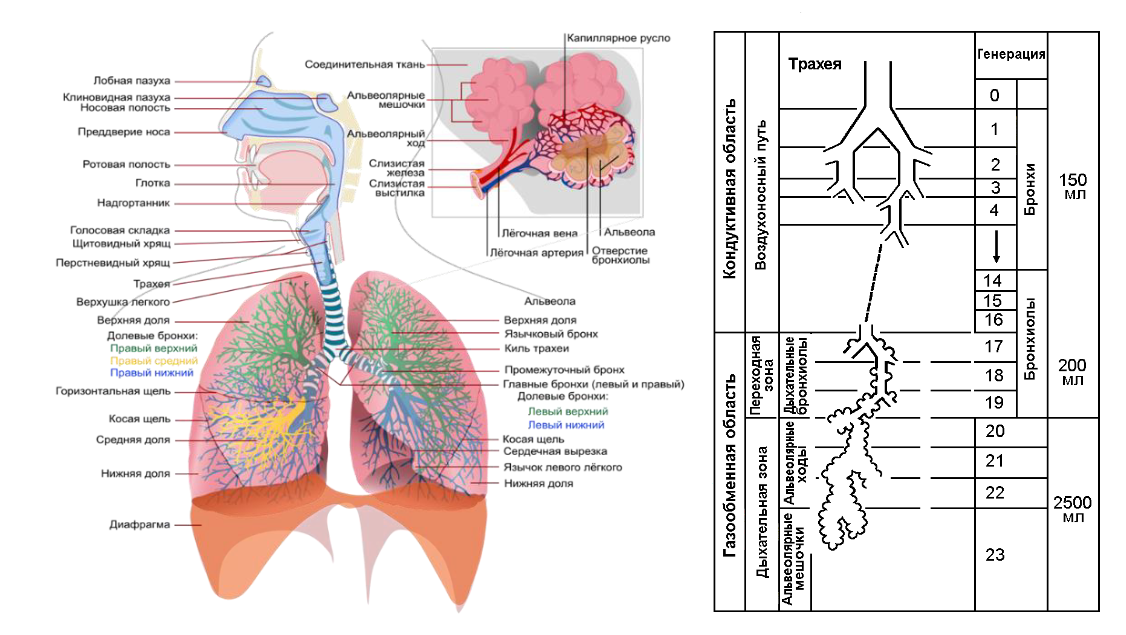
\includegraphics[width=\textwidth]{Система_органов.png}
                \caption{Система органов дыхания и поколение дыхательных путей.}
            \end{figure}

            Основной элемент, который занимается газообменом, в дыхательной
            системе является альвеола (рис. 2).

            \begin{figure}[h]
                \centering
                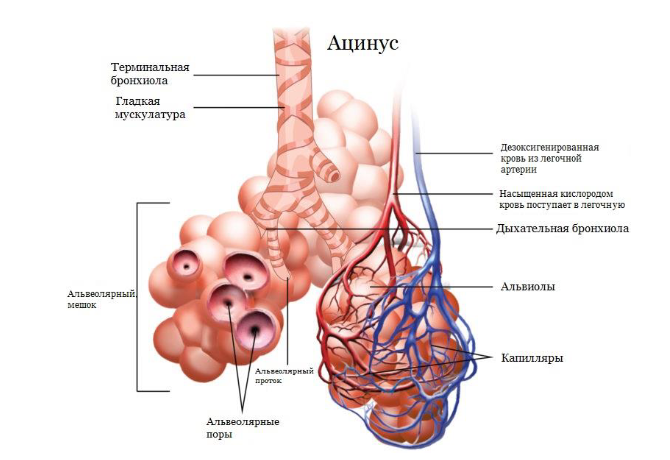
\includegraphics[width=0.65\textwidth]{Альвеолы.png}    
                \caption{Структура альвеолы.}
            \end{figure}

            Альвеолы представляют собой полые мешочки, имеющие открытые концы,
            продолжающиеся с просветами воздухоносных путей. Внутренние стенки
            выстланы одним слоем плоских эпителиальных клеток, называемых
            альвеолярными клетками первого типа, с вкраплениями более толстых
            специализированных клеток, называемых альвеолярными клетками второго
            типа. Альвеолярные стенки содержат капилляры и небольшое интерстициальное
            пространство с интерстициальной жидкостью и соединительной тканью. Кровь
            внутри капилляра альвеолярной стенки отделена от воздуха внутри альвеолы
            очень тонким барьером. В стенках также есть поры, которые пропускают воздух.
            Большая площадь поверхности и тонкий барьер позволяют быстро обменивать
            большие количества кислорода и углекислого газа путем диффузии.
            \vspace*{4mm}

            Стоит отметить, если у нас присутствует зона конвекции и зона
            диффузия, то в организме присутствует «мертвое пространство». Данное
            пространство названо из-за того, что в нем не происходит как раз газообмена. \\

            Функции «мёртвого пространства»:

            \begin{itemize}
                \item Воздух, заполняющий «мертвое пространство», играет роль буфера,
                который сглаживает колебания состава альвеолярного газа в ходе
                дыхательного цикла.

                \item Кондиционирование вдыхаемого воздуха за счет интенсивного
                кровоснабжения и секреции слизистой оболочки носовых ходов,
                носоглотки, гортани, трахеи и бронхов.
            \end{itemize}
        
            В свою очередь, «мёртвое пространство» можно разделить на
            анатомическое и функциональное. В первом случае, изначально
            организмом не предполагалось газообмена, а во втором случае,
            пространство, которое потеряло функцию газообмена из-за каких-либо
            причин (курение, вдыхание строительной пыли и тд.)
            \newpage

        \addcontentsline{toc}{subsubsection}{Механизм инспирации}
        \subsubsection*{Механизм инспирации}

            \hspace*{4mm} В процессе вдоха происходит сокращение мышц, прикрепленных к ребрам
            с внешней стороны, что вытягивает ребра и приводит к расширению грудной
            полости (рис. 3). Далее диафрагма сокращается, перемещается вниз и
            расширяет грудную полость, что приводит к сокращению мышц живота.
            Расширение грудной полости создает частичный вакуум, который всасывает
            воздух в легкие и заполняет расширенные альвеолы.            
            \vspace*{4mm}

            Процесс вдоха:

            \begin{enumerate}
                \item Процесс поступления атмосферного воздуха известен как вдох. Это
                активный процесс.

                \item При увеличении объема грудной полости и уменьшении давления
                воздуха происходит вдох.

                \item Сокращение наружных межреберных мышц увеличивает объем грудной
                полости.

                \item Сокращение диафрагмы еще больше увеличивает объем грудной
                деятельности. Одновременно легкие расширяются.

                \item По мере расширения легких давление воздуха внутри легких снижается.
                
                \item Давление выравнивается и атмосферный воздух устремляется внутрь
                легких.
            \end{enumerate}

        \addcontentsline{toc}{subsubsection}{Механизм экспирации}
        \subsubsection*{Механизм экспирации}

        \hspace*{4mm} Процесс выдоха считают один раз после того, как в легких происходит
        газообмен и вытесняется воздух. Этот выброс воздуха называется выдохом. Во
        время этого процесса мышцы, прикрепленные к ребрам, сокращаются, мышцы
        диафрагмы и живота расслабляются, что приводит к уменьшению объема
        грудной полости и увеличению давления в легких, в результате чего воздух в
        легких выталкивается наружу.
        \vspace*{4mm}

        Процесс выдоха:

        \begin{enumerate}
            \item Процесс выдоха углекислого газа называется выдохом. Это пассивный
            процесс.

            \item Это происходит, когда уменьшается размер грудной клетки и
            увеличивается давление воздуха снаружи.

            \item Теперь наружные межреберные мышцы расслабляются, а внутренние
            сокращаются.

            \item В результате ребра подтягиваются внутрь и размеры грудной полости
            уменьшаются.

            \item Диафрагма расслабляется, а легкие сжимаются.
            
            \item В результате давление увеличивается, и воздух вытесняется наружу.
        \end{enumerate}

        \begin{figure}[h]
            \centering
            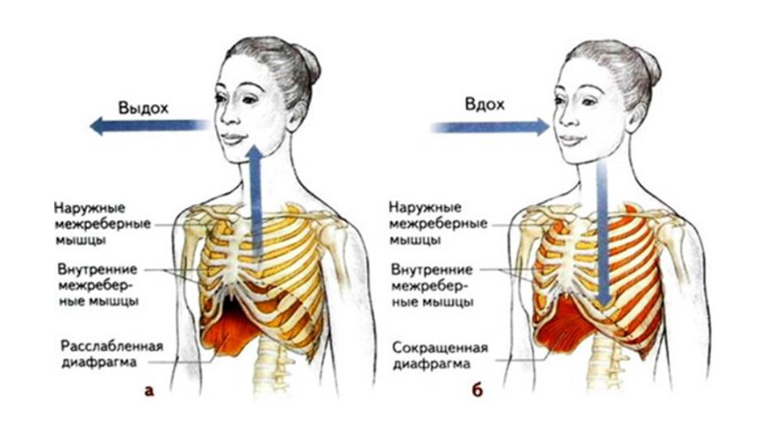
\includegraphics[width=\textwidth]{Инспирация_Экспирация.png}
            \caption{Механизм инспирации и экспирации.}
        \end{figure}
        \newpage

        \addcontentsline{toc}{subsubsection}{Структура лёгкого}
        \subsubsection*{Структура лёгкого}

            \hspace*{4mm} Каждое легкое окружено закрытым плевральным мешком, состоящим из
            тонкого листка клеток, называемого плеврой. Плевральная поверхность,
            покрывающая легкое (висцеральная плевра), прикрепляется к легкому
            соединительной тканью (рис. 4). Наружный слой (париетальная плевра)
            прикрепляется к грудной стенке и диафрагме. Тонкий слой внутриплевральной
            жидкости разделяет два слоя плевры. Изменения гидростатического давления
            внутриплевральной жидкости – внутриплеврального давления или
            внутригрудного давления заставляют легкие и грудную стенку сближаться и
            сближаться во время дыхания.

            \begin{figure}[h]
                \centering
                \includegraphics*[width=0.8\textwidth]{Плевра.png}
                \caption{Пример изображения плевры.}
            \end{figure}

            Плевральное и транспульмональное давление поддерживают легкие в
            раскрытом состояние. Другими словами, не дают легким привести к полному
            сжатию или наоборот коллапсу.
            \newpage

        \addcontentsline{toc}{subsection}{Спирометрия и спирография}
        \subsection*{Спирометрия и спирография}

            \hspace*{4mm} \textbf{\textit{Спирометрия}} — один из наиболее доступных и полезных тестов функции
            легких. Он измеряет объем воздуха, выдыхаемого в определенные моменты
            времени во время полного выдоха с силой, которому предшествует
            максимальный вдох.
            \vspace*{4mm}

            В свою очередь, \textbf{\textit{спирография}} является той же методикой, что и
            спирометрия, однако используется дополнительное оборудования для обработки
            выходных данных в виде графических изображений.
            \vspace*{4mm}

            Наиболее важные переменные, о которых сообщается, включают общий
            объем выдоха, известный как форсированная жизненная емкость легких, объем
            выдыхаемого воздуха за первую секунду, известный как объем форсированного
            выдоха за одну секунду, и их соотношение. Эти результаты представлены на
            графике в виде объемов и комбинаций этих объемов, называемых емкостью, и
            могут быть использованы в качестве диагностического инструмента, как
            средство наблюдения за пациентами с легочными заболеваниями.


    \addcontentsline{toc}{section}{Ход работы}
    \section*{Ход работы}

        \addcontentsline{toc}{subsection}{Оборудование}
        \subsection*{Оборудование}

            \hspace*{4mm} В данной работе для исследования использовался компьютерный
            спирометр (рис. 5) пневмотахометрического типа от компании «Нейрософт».

            \begin{figure}[h]
                \centering
                \includegraphics*[width=0.75\textwidth]{Спирометр.png}
                \caption{Спиро-спектр компании «Нейрософт»}
            \end{figure}
        \newpage

        \addcontentsline{toc}{subsection}{Наблюдения}
        \subsection*{Наблюдения}
            
            \hspace*{4mm} Исследование проводилось со студентом 19 лет, имеющего небольшой стаж курения.
            Было проведено два измерения: определение жизненной ёмкости лёгких (ЖЕЛ) и 
            определение максимальной вентиляции лёгких (МВЛ).
            \vspace*{4mm}

            В первом измерении (рис. 6) в спокойном состоянии было сделано 3 вдоха/выдоха, а затем
            глубокий вдох с последующим выдохом.
            \vspace*{4mm}

            \begin{figure}[h]
                \centering
                \includegraphics*[width=\textwidth]{ЖЕЛ.jpg}
                \caption{Спирограмма определения ЖЕЛ.}
            \end{figure}

            Ряд параметров, вычисленных при помощи компьютерной программы:

            \begin{center}
                \begin{tabular}{|l|l|}
                    \hline
                    Параметр & Значение \\ \hline
                    ЖЕЛ, л & 6.11 \\ \hline
                    ДО, л & 1.80 \\ \hline
                    РО{выдх}, л & 2.76 \\ \hline
                    РО{вдх}, л & 1.54  \\ \hline
                \end{tabular}
            \end{center}

            Где ДО - \textit{дыхательный объём}. Это общее количество воздуха, вдыхаемого
            или выдыхаемого при обычном расслабленном состоянии. РО{выдх} - под \textit{резервным объёмом выдоха} понимается
            дополнительная ёмкость воздуха, которую можно принудительно выдохнуть после истечения
            стандартного дыхательного объёма. РО{вдх} - \textit{резервный объём вдоха}. Это дополнительный
            объём, который можно эффективно вдохнуть после вдоха стандартного
            дыхательного объёма.

            \begin{figure}[h]
                \centering
                \includegraphics*[width=0.75\textwidth]{СоотношенияСпирограммы.png}
                \caption{Соотношения параметров на спирограмме}
            \end{figure}

            \hspace*{4mm} Во втором измерении (рис. 8) было сделано сначала 3 вдоха/выдоха
            при спокойном дыхании, а затем столько же при интенсивном.
            \vspace*{4mm}

            Ряд параметров, вычисленных при помощи компьютерной программы:

            \begin{center}
                \begin{tabular}{|l|l|}
                    \hline
                    Параметр & Значение \\ \hline
                    МВЛ, л & 79.11 \\ \hline
                    ДО{сп}, л & 1.21 \\ \hline
                    ДО{мвл}, л & 4.64 \\ \hline
                    ЧД, 1/мин & 14.00  \\ \hline
                    Время МВЛ, с & 12.00 \\ \hline
                \end{tabular}
            \end{center}

            Где ДО{сп} и ДО{мвл} - дыхательные объёмы в спокойном состоянии и при максимальной
            вентиляции лёгких соответственно. ЧД - \textit{частота дыхания}.

            \begin{figure}[h]
                \centering
                \includegraphics*[width=\textwidth]{МВЛ.jpg}
                \caption{Спирограмма определения МВЛ.}
            \end{figure}
        \newpage

    \addcontentsline{toc}{section}{Обработка данных}
    \section*{Обработка данных}

        \hspace*{4mm} Известно, что общая ёмкость лёгких (ОЕЛ) складывается из ЖЕЛ и остаточного объёма (ОО).
        
        \begin{center}
            ОЕЛ = ЖЕЛ + ОО
        \end{center}

        Где ЖЕЛ и ОО составляют 80\% и 20\% от ОЕЛ.
        \vspace*{4mm}

        Решив пропорцию, находим ОО и ОЕЛ:\\
        \\
        ОЕЛ = 7637.5 мл. \\
        ОО = 1527.5 мл. \\

        В нормальном спокойном состоянии ОО должно приблизительно находиться
        в пределах от 1100 мл до 1200 мл. Величина отклонения составляет приблизительно
        377.5 мл.
        \vspace*{4mm}
        \newpage

        Для оценки дыхания также можно вычислить \textit{функциональную остаточную ёмкость} (ФОЕ).
        ФОЕ - это общий объём воздуха, находящийся в лёгких после процесса выдоха. Ещё данная ёмкость
        называется альвеолярной. Другими словами, это те объёмы, которые остаются в альвеолах лёгких и воздухоносных
        путях.

        \begin{center}
            ФОЕ = РО{вдх} + ОО
        \end{center}

        ФОЕ = 3067.5 мл. В нормальном состоянии ФОЕ должен быть приблизительно
        равен 2400 мл. Величина отклонения составляет 667.5 мл.
        \vspace*{4mm}

        Также можно найти \textit{минутный объём дыхания} (МОД).
        МОД - это объём воздуха, который можно вдохнуть/выдохнуть из
        лёгких человека за минуту.

        \begin{center}
            МОД = ДО$\times$ЧД
        \end{center}
        Для спокойного дыхания МОД = 16.94 л/мин.\\
        При интенсивном дыхании МОД = 64.96 л/мин.
        \vspace*{4mm}

        \hspace*{4mm} В нормальном спокойном состоянии МОД должен приблизительно находиться
        в пределах от 5 л до 8 л. Величина отклонения в среднем составляет 10.44 л/мин.
        \vspace*{4mm}
        
        Ещё одной важной характеристикой является \textit{минутная альвеолярная вентиляция} (МАВ).
        МАВ - это тесно связанная величина с МОД. Это то количество воздуха/газа, которое
        доходит до альвеол за то же время, то есть минуту.

        \begin{center}
            МАВ = (ДО - АМП)$\times$ЧД
        \end{center}

        Где АМП - анатомически мёртвое пространство. АМП $\approx$ 140-160 мл.
        \vspace*{4mm}
        \\
        Для спокойного дыхания МАВ = 14.84 л/мин. \\
        При интенсивном дыхании МАВ = 62.86 л/мин.
        \vspace*{4mm}

        Последней рассматриваемой характеристикой будет \textit{коэффициент вентиляции лёгких} (КВЛ).
        КВЛ - показывает часть альвеолярного объёма, воздух которого
        обновляется за один вдох.\\

        КВЛ может быть вычислен по формуле:
        
        \begin{center}
            КВЛ = (ДО - АМП)/ФОЕ
        \end{center}

        КВЛ $\approx$ 0.35. В норме КВЛ должен быть численно приблизительно седьмой частью от ФОЕ.
        ФОЕ/7 $\approx$ 0.44. Величина отклонения составляет 0.09
    \newpage

    \addcontentsline{toc}{section}{Результаты и выводы}
    \section*{Результаты и выводы}

        \hspace*{4mm} В данной работе было проведено исследование дыхательных характеристик человека
        с использованием спирометрических методов. Был вычислен ряд величин, таких как ЖЕЛ, ФОЕ,
        ОЕЛ, МОД, МВЛ, МАВ и КВЛ. В результатах местами наблюдались отклонения от средних значений.
        Это связано, во-первых, с нечистотой эксперимента. Во-вторых, присутствует хоть небольшое, но влияние курения у испытуемого.
        Основной причиной, связанной с отклонениями, является недостаток проведённых испытаний, что явно увеличило
        погрешность всех последующих вычислений.
        
\end{document}